% !TEX program = xelatex

\documentclass[letterpaper,10pt,twoside]{article}
\usepackage{amsmath, amssymb, amsfonts, amsthm, bm, tensor}
\usepackage{mathtools, mathrsfs}
\usepackage{graphicx, fancyhdr}
\usepackage{xcolor, listings, hyperref, lastpage, doi, url}
\usepackage[left=1.in, right=1.in, top=1.5in, bottom=1.in]{geometry}
\usepackage{booktabs, siunitx}

%%%%%%%%%%%%%%%%%%%%%%%%%%%%%%%%%%
% Setup the bibliography package
\usepackage[style=authoryear, backend=biber, natbib=true]{biblatex}
\setlength\bibitemsep{1.5\itemsep}
\addbibresource{refs.bib}

%%%%%%%%%%%%%%%%%%%%%%%%%%%%%%%%%%
% Setup the header and the footer
% first I'll make some colors
\definecolor{gugray}{HTML}{666666}
\definecolor{gured}{HTML}{9a3b26}
\definecolor{gublue}{RGB}{0,63,114}

% Add a rule across the top and bottom
\renewcommand{\headrule}{{\color{gugray}%
  \hrule width\headwidth height\headrulewidth \vskip-\headrulewidth}}
\renewcommand{\footrule}{{\color{gugray}%
  \vskip-\footruleskip\vskip-\footrulewidth%
\hrule width\headwidth height\footrulewidth\vskip\footruleskip}}
\renewcommand{\headrulewidth}{1.0pt}
\renewcommand{\footrulewidth}{1.0pt}

\pagestyle{fancy}

% specify what to put in each header box
\lhead{\color{gublue}}
\chead{\color{gublue}ENSC 481}
\rhead{}
\lfoot{}
\cfoot{\color{gugray}\thepage}
\rfoot{}


%%%%%%%%%%%%%%%%%%%%%%%%%%%%%%%%%%
% setup Listings Package from Matlab:
\definecolor{matcolor_comment}{rgb}{0.13333333,0.54509804,0.13333333}
\definecolor{matcolor_keyword}{rgb}{0,0,1}
\definecolor{matcolor_strings}{rgb}{0.62745098,0.12549020,0.94117647}
\lstset{language=Matlab,
frame=ltrb,framesep=5pt,basicstyle=\ttfamily\normalsize,
numbers=left,
identifierstyle=\color{black},
keywordstyle=\color{matcolor_keyword},
stringstyle=\color{matcolor_strings},
commentstyle=\color{matcolor_comment}}

%%%%%%%%%%%%%%%%%%%%%%%%%%%%%%%%%%
% These are some macros to make vectors/matrices Dr Fitz style
\providecommand\Vec{}
%\renewcommand{\Vec}[1]{ \vec{#1} }
\renewcommand{\Vec}[1]{ \bm{#1} }
% Unit vector
\newcommand{\uVec}[1]{ \hat{\bm{#1}} }
% 2nd order Tensor
\newcommand{\Ten}[1]{ \bm{#1} }
% 4th order Tensor
\newcommand{\TenF}[1]{ \bm{\mathfrak{#1}} }
% Colum Vector
\newcommand{\Col}[1]{ \bm{\mathsf{#1}} }
% Matrix
\newcommand{\Mat}[1]{ \bm{ \mathsf{ #1 }} }


%%%%%%%%%%%%%%%%%%%%%%%%%%%%%%%%%%
% Stuff for the title block
\title{Example of using \LaTeX}
\date{9 Feb 2021}
\author{T. Fitzgerald}


%%%%%%%%%%%%%%%%%%%%%%%%%%%%%%%%%%
% Start the document
\begin{document}

% Print the title
\maketitle

% Print the table of contents
\tableofcontents

%--------------------------------------------------------------
\section{Section title}
Welcome to wild and wonder world of \LaTeX , where the syntax is made-up and points don't matter.
I've put each new sentence on its own line in the original file, as this helps with using version--control systems, like git.
However, in the compiled document all these sentences show up as a single paragraph.

To get a new paragraph, I need to add an extra blank line like this.
Once we get over the simple parts, writing up something in \LaTeX\ is actually fun.
Using a good editor\footnote{I'm using \href{https://code.visualstudio.com/}{VS Code} locally with the \href{https://marketplace.visualstudio.com/items?itemName=James-Yu.latex-workshop}{LaTeX Workshop} Extension.  On Windows I like to install and manage \LaTeX\ using \href{https://miktex.org/}{MikTeX}.} %
helps to smooth over the bumps.
I think the best parts of using \LaTeX\ over other document preparation systems are
\begin{enumerate}
  \item It's structured.  
  We can make sections, subsection, subsubsections, chapters and parts (if we're in the right documentclass) and it will automatically keep all the internal booking for us.
  
  \item Math looks great.  
  Once we get over the syntax of writing math, it's hard to use anything else.\footnote{Perhaps this is just because I'm snooty.}  
  In all seriousness, when the math is clear and consistent it is not distracting.
  
  \item Figures can be pdfs and therefore can be vector graphics.  
  We make a use lots of line graphics, so the ability to make figures that aren't blurry is very powerful.

  \item Citations are easy.  
  I make a bibliography file using \href{https://www.jabref.org/}{JabRef}, and then I just need to add a \texttt{citet} or \texttt{citep} in my text and I'm done.
  \begin{itemize}
    \item A direct reference: For example, \citet{Akhtaruzzaman2010} show several examples of controlling the rotary inverted pendulum.
    The classical treatise \citet{Goldberg1991} on floating--point arithmetic

    \item A parenthetical cite: Dense eigenvalue computations can be very robust \citep{Golub2012}.
  \end{itemize}
\end{enumerate}

%--------------------------------------------------------------
\subsection{Math}
In the Matlab example I plot the following function
\begin{align}
    f(t) = \sin\left( 2\pi \left( \frac{c}{2}t^2 + f_0 t \right) \right)
\end{align}

%--------------------------------------------------------------
\subsection{Graphics}

I'm using the \texttt{graphicx} package to add a pdf into this example.
We can see the results in Figure \ref{fig:func1}.
The code to produce this figure is provided in \S\ref{sec:code}.

\begin{figure}[h!] % the [h!] means "put it here and don't float it around"
    \centering
    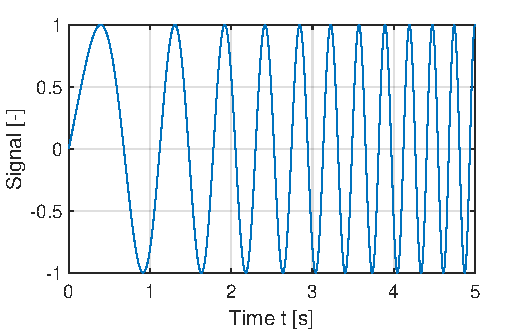
\includegraphics[scale=1]{chirp}
    \caption{This a cool function}
    \label{fig:func1}
\end{figure}

\subsection{Some notation}

To demonstrate some of the flexability of the math fonts I've written out Table \ref{tab:notation}.
It also shows building a table using the \texttt{tabular} package.

\vspace{24pt}
\begin{table}[h!]
   \centering
   \caption{Summary of the notation convention for math quantities}
   \label{tab:notation}
\begin{tabular}{lccl}
  \toprule
  \textbf{Quantity} & \textbf{Group} & \textbf{Symbols} & \textbf{Notes}\\
  \midrule
  scalar & $\mathbb{R}$, $\mathbb{C}$, or $\mathbb{Z}$ & $a,\, b,\, c,\, \ldots$ & italics, upper and lower case \\
          &                                             & $\alpha,\, \beta,\, \gamma ,\, \ldots$ & Greek and Latin \\
  \midrule
  vector (order 1 tensors) & $\mathbb{E}^3$ &  $\Vec{a},\, \Vec{b},\, \Vec{c},\, \ldots$ & lower case, bold italics \\
  2${}^\text{nd}$ order tensor & $\text{Lin}\coloneqq \mathcal{L}\left(\mathbb{E}^3,\mathbb{E}^3 \right)$ & $\Ten{A},\, \Ten{B},\, \Ten{C} \ldots$ & upper case, bold italics \\
  4${}^\text{th}$ order tensor & $\mathcal{L}\left(\text{Lin},\text{Lin}\right)$ & $\TenF{A},\, \TenF{B},\, \TenF{C},\, \ldots$ & upper case, bold Fraktur \\
  \midrule
  $n$--tuple & $\mathbb{R}^n$ & $\Col{a},\,\Col{b},\,\Col{c},\, \ldots$ & lower case, bold, sans serif \\
  matrix & $\mathbb{R}^{n\times m}$ & $\Col{A},\,\Col{B},\,\Col{C},\, \ldots$ & upper case, bold, sans serif \\
  \bottomrule
\end{tabular}
\end{table}

%--------------------------------------------------------------
\section{Further reading}
Some more topics to look into include
\begin{itemize}
    
    \item Making \href{https://en.wikibooks.org/wiki/LaTeX/Tables}{tables} can be a little tricky at first.

    \item Managing citations and a bibliography\footnote{This is a nice article \url{https://www.overleaf.com/learn/latex/bibliography_management_with_bibtex}}
    
    \item Working with more types of math can get involved.\footnote{Overleaf is good here, but here is another point of reference \url{https://en.wikibooks.org/wiki/LaTeX/Advanced_Mathematics}}

\end{itemize}


%--------------------------------------------------------------
\section{Code Example}
\label{sec:code}

Below I'm using the \href{https://ctan.org/pkg/listings?lang=en}{\texttt{listings}} package to insert the Matlab code that generated Figure \ref{fig:func1}.
I've modified the Matlab language definition in the header of this file to make the colors, font, and line numbering the way I prefer it.

\lstinputlisting[language=Matlab]{make_figure.m}


%--------------------------------------------------------------
% Insert the bibliography
\printbibliography

\end{document}